\documentclass[runningheads]{llncs}

\usepackage[utf8]{inputenc}
\usepackage[T1]{fontenc}
\usepackage{graphicx}
\usepackage{subcaption}

\usepackage{amsmath}
\usepackage{mathtools}

\begin{document}

\title{Music Emotions Classification: A General Model Fine-Tuned On User}



\author{Francesca Gasparini\orcidID{0000-0002-6279-6660} \and
Mattia Marchi}

\authorrunning{F. Gasparini and M. Marchi}
\institute{Department of Informatics, Systems and Communication,\\
University of Milano-Bicocca, Milano, Italy\\
\email{francesca.gasparini@unimib.it}\\
\email{m.marchi@campus.unimib.it}}


\maketitle

\begin{abstract}
This paper presents an approach for music emotion recognition (MER) using deep learning algorithms. MER systems nowadays can have different uses, from the generation of customized playlists based on the user's mood to the musical suggestions implemented by musical streaming platforms. The proposed model consists in a state-of-the-art Convolutional Neural Network (CNN) to extract the main features from Mel spectrograms, generated by music files, and a Long Short-Term Memory (LSTM) as a classifier. The class of emotions examined corresponds to Russell's four-quadrant. We have merged three datasets from the literature to create a model with a better generalization, achieving 91\% accuracy. We also studied the ability of the model to adapt to the individual user, implementing the possibility of fine-tuning the network on the emotions perceived by the user. The main objective is to create a model that is able to properly generalize and then to adapt it to the perceptions of each individual user, in order to consider the subjectivity of perception. The system was tested on three different users using 50 songs, showing an accuracy of predicted emotions of 44.68\% for the general model. User-tuned models that consider 10 and 20 user-suggested emotions reached an average of correctly predicted songs of 62.66\% and 76\% respectively, greatly improving the general model results and gradually decreasing the average prediction error.

\keywords{Music Emotion Recognition  \and Affective Computing \and Deep Learning \and Convolutional Neural Network \and  Long Short-Term Memory.}
\end{abstract}

\section{Introduction}
Users increasingly need contents filtered according to their interest. With this aim, several Recommender Systems (RS) have been developed, revolutionizing the way people enjoy the contents \cite{Konstan2012Apr}. Music is one of those fields where recommender systems have been recently applied. There is already a significant number of research works for music RS, using different types of data: audio signals, content-based information and ratings from users \cite{deep-re-sys-survey}. 
A further step in research is to improve recommender systems using the  user's emotions. The Music Emotion Recognition (MER) has become a fundamental aspect to guarantee the user a better subjective experience. MER systems have a large number of possible applications, such as automatic playlist generation and music suggestion application (Spotify, SoundCloud, ...). In this paper, we explore the possibility of creating a generalized model to recognize the mood provided by a song, using its Mel spectrogram \cite{demircan2020comparison}, and then adapt this model to the single user. To adapt the general model to the user, some of his/her explicit emotions referred to a dataset of songs are used to fine-tune the model on his/her emotional responses. The proposed approach is based on a Convolutional Neural Network (CNN) \cite{krizhevsky2012imagenet} combined with a Long Short-Term Memory (LSTM) \cite{hochreiter1997long}. 
There are several ways to classify emotions induced by a song, which can be grouped into two models: categorical and dimensional. Categorical models divide emotions into several groups of adjectives. One of the most used approaches has been introduced by Plutchick \textit{et al.} \cite{plutchik2013theories}, who divides emotions into 8 categories represented by a wheel of emotions. Dimensional approaches, on the other hand, label songs based on their position in a dimensional space. The most used representation, proposed by Russell \cite{Russel}, divides the space into three dimensions: arousal, valence and dominance. 
The model adopted in our work considers two dimensions (valence and arousal), classifying each song into one of the Russell's four-quadrants of this 2D space.
This paper is organized as follows. Section 2 introduces the state of the art of automatic music emotion recognition. In section 3 the three datasets used in this work are described. In section 4 the general MER model is presented and our user-tuned proposal is described. The experimental results are discussed in section 5. Eventually, conclusions and possible future works are included in section 5. 


\section{State Of The Art}

There are several approaches in the literature to model a MER system. The first of these approaches uses audio features directly obtained from the audio files and supplies them to a classifier. For instance, Han \textit{et al.} developed a multi-class Support Vector Machine classifier using only low-level features such as energy, zero crossing rate (ZCR), audio spectrum and wavelet \cite{han2010music}. The songs were classified on a wide range of emotional categorical classes (11 labels), such as "happy", "peaceful" and "bored". The study was performed using a very limited dataset of 120 songs. The results obtained showed an overall accuracy of 67.54\%.
A different point of view is provided by Liu \textit{et al.} through the combined use of LSTM, to classify the audio signals, and BERT, to obtain an estimate of the mood through the lyrics of the song \cite{liu2020research}. 
%The ensemble model scheme is shown in figure \ref{fig-Liu}. 
LSTMs have empirically shown an improvement in performance on audio signals compared to other machine learning models. On the other hand, BERT is a multi-layer bidirectional transformer encoder, developed by Google AI team in 2018 \cite{devlin2018bert}, which allows to classify the emotions of the lyrics. The use of lyrics allows to analyze with more precision what a song wants to communicate and therefore what mood it arouses. The model, trained on a set of 1000 songs, achieves an average accuracy of 79.70\%.

%\begin{figure}
%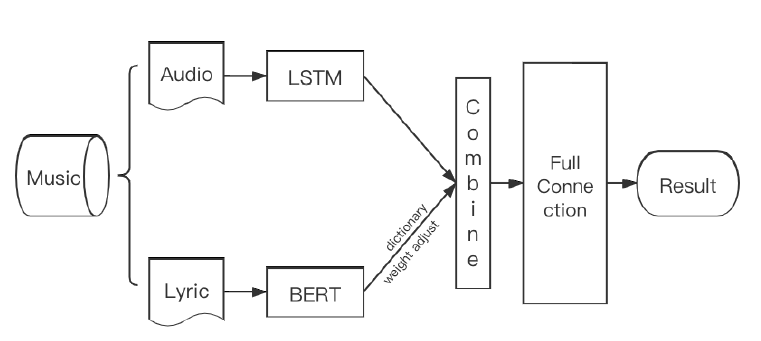
\includegraphics[width=\textwidth]{img/Liu_model.PNG}
%\caption{Ensemble model scheme\cite{liu2020research}.}
%\label{fig-Liu}
%\end{figure}



With research improvements and thanks to some famous contests like \textit{ImageNet} \cite{krizhevsky2012imagenet}, the CNNs have become more and more popular in music classification. CNN networks allow to use images generated from audio files, as the representation of signals, and to classify them with excellent performance results. Bahuleyan in 2018 has applied a CNN on images representing the Mel Spectrograms of the songs, with the aim of categorizing music files according to their genre \cite{bahuleyan2018music}. The CNN architecture used is the VGG-16 \cite{simonyan2014very}, one of the top performing model in \textit{ImageNet} Challenge in 2014. The dataset used contained a large number of audio files (40540), divided into 7 genres. The study tested the pre-trained model in two different settings: transfer learning and fine-tuning. The best accuracy was achieved from the model fine-tuned, with an accuracy of 64\%.
In 2020, Hizlisoy \textit{et al.} studied how to classify the emotions aroused by listening to Turkish traditional songs, using the features obtained from a CNN and classifying them using a LSTM plus a Deep Neural Network (DNN) \cite{hizlisoy2021music}. The Turkish music database is composed of only 124 excerpts with a duration of 30 seconds. The music was annotated on 3 class emotions, based on valence and arousal. The performance of the combined LSTM + DNN model, applied to features extracted from CNN, has achieved an overall accuracy of 99.19 \%. 

\section{Datasets}
In order to achieve a better generalization, the proposed model  was obtained by combining three different datasets used in the MER field. The choice was made using three constraints: the audio files should be available, each excerpt should last at least 30 seconds and an emotional label should be associated with each excerpt. The three selected datasets are: \textit{PMEmo}\cite{zhang2018pmemo}, \textit{4Q}\cite{panda2018musical}\cite{panda2018novel} and \textit{Emotify}\cite{aljanaki2014collecting}\cite{aljanaki2016studying}.  In order to use the same emotional model for all datasets, the different annotations were properly converted into 4 classes corresponding to Russell's quadrants. The notation reported in table \ref{tab1} was used to label these quadrants. 
\begin{table}
\caption{Notation used to label Russell's quadrants.}
\label{tab1}
\centering
\begin{tabular}{|l|l|l|l|}
\hline
\textbf{Arousal} &  \textbf{Valence} & \textbf{Label} & \textbf{Quadrant}\\
\hline
Low &  Negative & 0 & A-V-\\
Low & Positive & 1 & A-V+\\
High & Negative & 2 & A+V-\\
High & Positive & 3 & A+V+\\
\hline
\end{tabular}
\end{table}


\subsection{PMEmo}

\textit{PMEmo}\footnote{https://github.com/HuiZhangDB/PMEmo} is a dataset publicly available for the research community, containing 794 songs, annotated by 457 subjects \cite{zhang2018pmemo}. In addition to the audio files, it also contains annotations relating to the physiological response of the participants listening to the songs. The 794 audio files correspond to the chorus of the first songs in several world listening music charts in 2016. In detail:
\begin{itemize}
    \item 487 songs from \textit{Billboard Hot 100};
    \item 616 songs from \textit{iTunes Top 100};
    \item 226 songs from \textit{UK Top 40 singles}.
\end{itemize}

The annotations related to the choruses have been released as a value between $[0, 1]$ of arousal and valence. The conversion performed is the following:
\begin{itemize}
    \item $(Arousal \le 0.5) \wedge (Valence \le 0.5) \to Label = 0$
    \item $(Arousal \le 0.5) \wedge (Valence > 0.5) \to Label = 1$
    \item $(Arousal > 0.5) \wedge (Valence \le 0.5) \to Label = 2$
    \item $(Arousal > 0.5) \wedge (Valence > 0.5) \to Label = 3$
\end{itemize}




In order to manage the choruses of variable length they have been converted to a fixed length of 30 seconds. %It is possible to notice in  figure \ref{fig-pmemo} how
The dataset is unbalanced, with a large number of songs with valence and arousal greater than $0.5$. For this reason, only a subset of 150 audio files have been used, in order to avoid an overly unbalanced training set. %750 Mel Spectrograms will be extracted from these files and used for training.

%\begin{figure}
%5\centering
%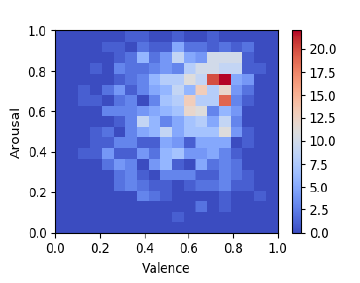
\includegraphics[scale = 0.6]{img/PMEmo_distribution_annotations.PNG}
%\caption{Distribution of annotations in PMEmo dataset\cite{zhang2018pmemo}.}
%\label{fig-pmemo}
%\end{figure}

\subsection{4Q}
\textit{4Q} dataset\footnote{http://mir.dei.uc.pt/downloads.html} contains 900 audio clips, with subjective annotations following Russell's emotion quadrants \cite{panda2018musical}\cite{panda2018novel}. Each clip has a duration of 30 seconds and files are organized in 4 folders, each containing 225 files, corresponding to the four quadrants. The songs are obtained by querying and filtering the \textit{AllMusic} API\footnote{http://developer.rovicorp.com}. The dataset is balanced, so all the excerpts are used in the final merged dataset.



\subsection{Emotify}

\textit{Emotify} dataset\footnote{http://www2.projects.science.uu.nl/memotion/emotifydata/} contains 400 songs, divided into 4 different musical genres: classical, electronic, pop and rock. The annotations were obtained through a game in which the participants labeled the emotions induced by the songs of different genres. Unlike previous datasets, \textit{Emotify} uses categorical emotion labeling, following the GEMS scale \cite{zentner2008emotions}. For each song, the number of votes for each emotion category are provided. We therefore used the emotion with the highest number of votes as a single label. In order to convert categorical emotions into the valence arousal model, we used the scheme reported in figure \ref{fig-emotify}. After this conversion, the dataset was extremely unbalanced, with most labels in the quadrant having low arousal and positive valence. Even in this case only 150 audio files were used in order to keep balanced the final dataset.

\begin{figure}
\centering
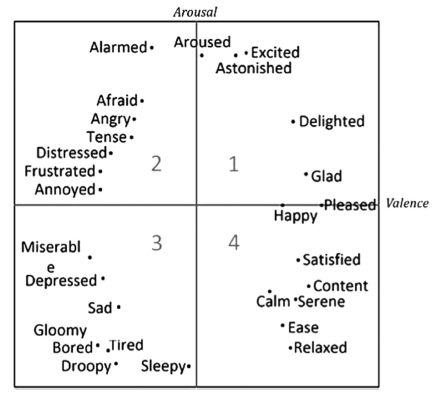
\includegraphics[scale = 0.48]{img/categorical-to-russell.PNG}
\caption{Russell circumplex with categorical emotions \cite{panda2018novel}.}
\label{fig-emotify}
\end{figure}

\subsection{Preprocessing}

Once the merged dataset is obtained, the final number of audio files is 1200 of 30 seconds duration.  Each file is divided into 5 frame of 6 seconds, obtaining 6000 frames. 
On these frames the MEL spectrogram is computed. The choice to use spectrograms was made because spectrograms are inclusive of para-lingual information and therefore useful for the tasks of recognizing emotions \cite{ma2018emotion}. The \textit{Librosa} python library was used to generate the spectrograms \cite{mcfee2015librosa}. An example of the generated spectrograms is shown in figure \ref{fig-spectrogram}.

The parameters used for the generation of the Mel spectrograms are:
\begin{itemize}
    \item \textbf{Sample Rate:} 22050;
    \item \textbf{Frame/Window size:} 2048;
    \item \textbf{Hop Size:} 512;
    \item \textbf{Number of Mel bins:} 96;
    \item \textbf{Size of Image:} 300 x 300 pixels.
\end{itemize}
The final dataset has been split into train, test and validation set with the respective percentage of 70\%, 15\% and 15\%. The split is done using the IDs of the audio file before the generation of the Mel spectrograms, in order to avoid having different frames of a song in different sets.


\begin{figure}
\centering
	\begin{subfigure}[t]{.4\textwidth}
         \centering
         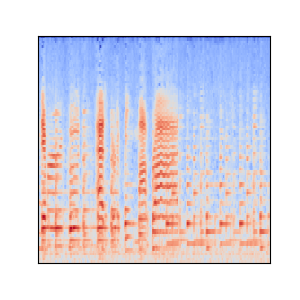
\includegraphics[scale = 0.4]{img/Mel-0.png}
         \caption{Low Arousal - Negative Valence}
	\end{subfigure}
	\quad
	\begin{subfigure}[t]{.4\textwidth}
		\centering
        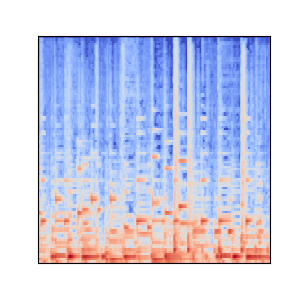
\includegraphics[scale = 0.4]{img/Mel-1.png}
        \caption{Low Arousal - Positive Valence}
	\end{subfigure}
	
		\begin{subfigure}[t]{.4\textwidth}
         \centering
         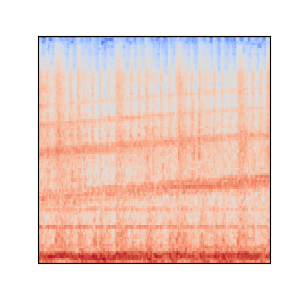
\includegraphics[scale = 0.4]{img/Mel-2.png}
         \caption{High Arousal - Negative Valence}
	\end{subfigure}
	\quad
	\begin{subfigure}[t]{.4\textwidth}
		\centering
        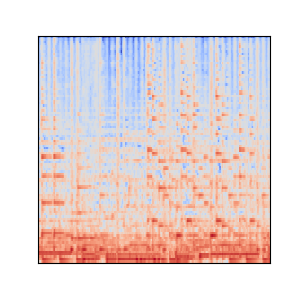
\includegraphics[scale = 0.4]{img/Mel-3.png}
        \caption{High Arousal - Positive Valence}
	\end{subfigure}
	\caption{Example of 4 different spectrograms corresponding to audio files of different emotional classes.}
	\label{fig-spectrogram}
\end{figure}




\section{MER Models}
The model we propose to solve the general music emotion recognition task consists of two fundamental components:
\begin{itemize}
    \item Convolutional Neural Network (CNN);
    \item Long Short-Term Memory (LSTM).
\end{itemize}
These models are described in section 4.1 and 4.2 respectively.
In particular we fine tuned pre-trained CNNs in order to learn  characteristics of Mel
spectrograms, relevant in a MER task. Then, from these CNNs, features are extracted to feed a classifier based on LSTM. 
Staring from this general model, we here propose to user-tuned it in order to better fit the emotions of each single user. Our proposal is described in section 4.3.

\subsection{Convolutional Neural Network}
The first model adopted to classify emotions using Mel spectrograms is a 3D convolutional network. This network is capable of understanding some characteristic patterns belonging to different emotional classes, considering the spectrograms as images \cite{bahuleyan2018music}. Two different state of the art networks are here considered and compared, and fine-tuning is applied with respect to the MER task:  %Fine tuning is a process in which the starting network is already pre-trained and allowing it to change its weights to learn a new taks.

\begin{itemize}
    \item \textbf{EfficientNet-B3} \cite{tan2019efficientnet}: this network presented in 2019 uses a scaling method that uniformly scales all dimensions of depth, width and resolution.
    \item \textbf{MobileNetV3-Large} \cite{howard2019searching}: Lightweight state of the art CNN with one of the best ratios between accuracy and speed of inference.
\end{itemize}

Both models use ImageNet starting weights and the following layers
have been introduced:
\begin{itemize}
    \item Flatten layer;
    \item Dense layer of 1024 output nodes, ReLu activation and L2 regularization with $\alpha = 0.1$;
    \item Dropout layer with dropout rate of 0.5;
    \item Dense layer of 512 output nodes, ReLu activation and L2 regularization with $\alpha = 0.1$;
    \item Dropout layer with dropout rate of 0.4;
    \item Dense layer of 128 output nodes, ReLu activation and L2 regularization with $\alpha = 0.1$;
    \item Dropout layer with dropout rate of 0.3;
    \item Dense layer of 4 output with softmax activation.
\end{itemize}
The objective function minimizes the \textit{sparse categorical crossentropy loss}, and is optimized with \textit{Adam} \cite{kingma2014adam}, with a training phase of 50 epochs and a batch size of 32 instances. In order to have the model with the best ability to generalize, we use the model weights that have obtained the best accuracy score on the validation set in the epochs. As shown in table \ref{tab2}, the model based on MobileNetV3 has a slightly lower accuracy, but with an average training time of about one third of EfficientNet-B3. Ideally, the application of recommender systems that we are studying should be able to run on users' mobile devices, so it is important to take into account the weight of the model. For this reason the network chosen in the final model is MobileNetV3.

\begin{table}
\caption{Performance of the CNN models.}
\label{tab2}
\centering
\begin{tabular}{|l|c|c|c|c|}
\hline
\textbf{Model} &  \textbf{Accuracy} & \textbf{F-score}  & \textbf{Average Training Time per Epoch}\\
\hline
\textbf{EfficientNet-B3} &  0.69  & 0.67 & 90s\\
\textbf{MobileNetV3} &  0.60 & 0.60 & 32s\\
\hline
\end{tabular}
\end{table}


\subsection{Long Short-Term Memory}

Once CNNs have been trained to understand the relevant characteristics of Mel spectrograms they can be used to perform features extraction. The model used as classifier is the Long Short-Term Memory (LSTM) \cite{hochreiter1997long}. LSTM is widely used in music recognition tasks due to its ability to process sequential information. 
To have the network capable of making inference on a song portion 24 seconds long, we consider 4 spectrograms, each corresponding to 6 seconds.
We feed the  pre-trained MobileNetV3 with these spectrograms and we extract the corresponding features from the last convolutional layer, flattened and reshaped to be considered a single input of 4 sequences for the LSTM, as shown in figure \ref{fig-train-lstm}. 



\begin{figure}
\centering
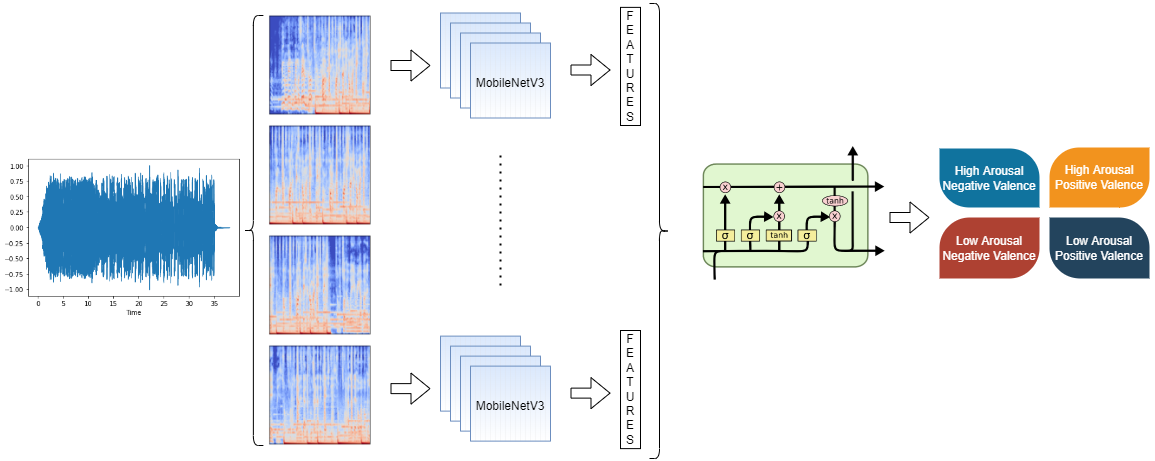
\includegraphics[scale = 0.5]{img/LSTM-Training.png}
\caption{Features are extracted using CNN from the input spectrograms and reshaped to be a single input of 4 sequences for LSTM.}
\label{fig-train-lstm}
\end{figure}

Specifically, the LSTM network is composed of:
\begin{itemize}
    \item LSTM layer of 128 hidden units, ReLu activation;
    \item Dropout layer with dropout rate of 0.2;
    \item Dense layer of 4 output with softmax activation.
\end{itemize}
The objective function minimises the \textit{sparse categorical crossentropy loss}, and is optimized with \textit{RMSprop} \cite{tieleman2012rmsprop}, with a training phase of 20 epochs and a batch size of 32 instances. As in the case of CNN, we use the model weights that have obtained the best accuracy score on the validation set in the epochs. The network achieves excellent results, with an accuracy and F-score of 0.91\%. As shown in the confusion matrix in figure \ref{Conf-train-lstm} there are very few wrong classifications.

\begin{figure}
\centering
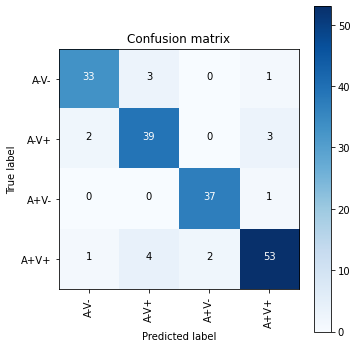
\includegraphics[scale = 0.48]{img/confusion-matrix-lstm.png}
\caption{Confusion matrix obtained on the test set.}
\label{Conf-train-lstm}
\end{figure}



\subsection{User-Tuned Model}
The main purpose of this paper is not only to find a model that is able - in general - to understand the emotions induced by the music, but also to adapt it to the individual user in case he had a different way of perceiving songs. The idea is to simulate a real context of integration of our model in an existing playlist generation system. 
In order to solve this problem, 50 new songs have been chosen from different genres and of variable length, with an average length of 280 seconds. The songs were chosen from the most famous ones for each genre, in order to simulate a real playlist of a user. The songs have been played for 3 different users and individually labeled, asking them to select the emotion felt from the quadrant of the arousal-valence model, as previously reported in figure \ref{fig-emotify}. The user could also explicitly indicate some emotions, which he/she wants the model to be aware of. 
Starting from the data labelled by each subject, our proposed user-tuned classifier can be described as follows. %When the user makes an emotion explicit to the model, a user fine-tuning process is made: 
The spectrograms,  corresponding to the entire songs are generated (evaluated for each 6-second frame), the features are extracted, they are labeled with the user's emotion and the model is user-tuned using the original dataset plus a portion of the new labeled data. The user-tuning of the classifier is applied starting from the pre-trained LSTM but with a very small learning rate (0.000001) through 50 epochs. This value was chosen empirically. The main purpose is to create a controlled overfitting in order to push the model towards the user's perception. This desired controlled overfitting effect is also obtained using a portion of the new generated spectrograms as validation set, in order to verify whether the network has learned the user's suggestion. The model will use the weights that have obtained the best accuracy on the validation set. The low learning rate is used to avoid excessive variation in the general model's weights and to avoid uncontrolled overfitting. 
The network will be able to recognize the emotions of the songs suggested by the user while remaining able to generalize. Applying this strategy, we obtained an average accuracy on the validation set of 89\%. The user-tuning process is outlined in figure \ref{fig-finetuning-process}.

\begin{figure}
\centering
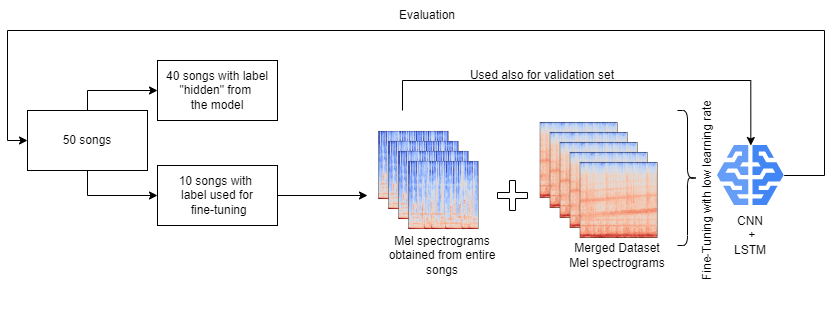
\includegraphics[scale = 0.45]{img/finetuning-process.png}
\caption{Summary of the user-tuning process.}
\label{fig-finetuning-process}
\end{figure}

\section{Results and Discussion}

The proposed user-tuned model is evaluated on a new dataset of 50 songs, obtained by asking 3 subjects to listen to the songs, label them and indicate 10 and 20 songs whose induced emotions he/she wants the model to be aware of. 
We thus create three user-tuned classifiers, one for each subject involved. 
We also compare two versions of the proposed classifiers, considering respectively the 10 and 20 suggested songs in the user-tuning step. 
Finally the performance of these user-tuned models are also compared with the general MER model previously described. 
To this end, each of the 50 new labelled songs are divided into frames of 24 seconds, to be classified by the LSTM. Thus for each song we obtain several emotional classes, one for each 24-second segment. Starting from the labels obtained for each segment, the final label is thus reported in terms of frequency (or percentage) of each of the 4 emotions, with respect to the whole song.      
A Python script was then created which, given as input the \textit{csv} file containing the user labels and the folder with the audio files, performs the following steps:
\begin{enumerate}
    \item Mel spectrograms are generated for 6 seconds of each song;
    \item Features are extracted from CNN as described in section 4.1 for each 24 seconds of each song, considering 4 spectrograms ;
    \item The features are reshaped and used as input to LSTM as described in section 4.2;
    \item LSTM generates several predictions, one for each 24-second sequence;
    \item A percentage estimate of all predictions is made, in order to consider the various mood changes within the song itself.
\end{enumerate}

A diagram of the algorithm is shown in figure \ref{fig-user-evaluation}. To quantify the performance of the classification we do not only consider the most frequent emotion, but we also introduce an error metric to quantify the distance between the results of the classification and the subject's labels, when the subject label has not been properly identified.  
This metric can be useful to understand how wrong the model is in the prediction. 
The proposed metric computes the difference between the frequency of the predicted emotion (the most frequent one in the classification output) and the frequency obtained for the true emotion class. 
Figure \ref{fig-output} reports an example for 5 songs (rows in the table) of the output of the user-tuned classifier, in terms of frequency of each emotional class, the corresponding class predicted by the classifier (column Max\_Overall\_Emotion), compared with the true label (User\_Emotion) and finally evaluating the error metric here proposed (Difference). 

\begin{figure}
\centering
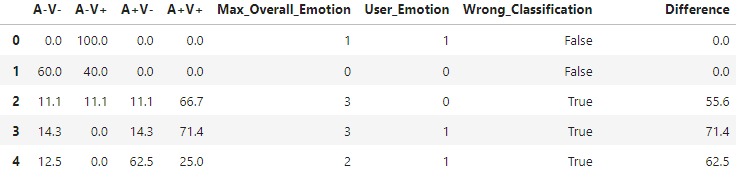
\includegraphics[scale = 0.62]{img/example-output.PNG}
\caption{Example of the result obtained on 5 songs after the execution of the model. The first 4 columns report the \textit{True\_Emotions} expressed by the user, with respect to the 4 quadrants of the arousal-valence plane. The corresponding quadrant is reported in column \textit{User\_Emotion}.  Column \textit{Max\_Overall\_Emotion} refers to the emotion quadrant with the highest percentage found by the model. If the two columns do not match, the prediction is considered wrong and the difference in estimates is calculated.}
\label{fig-output}
\end{figure}



%The average of the divergence of all the wrong predictions is then figured in the following way:
%\begin{equation}
%\begin{multlined}
%\forall \text{ wrong emotion}_i > \text{true emotion}_i: \\
%\frac{1}{n  = \text{Number Wrong Predictions}} \sum_{i}^n \text{wrong emotion}_i - \text{true emotion}_i
%\end{multlined}
%\end{equation}



The results obtained on the 50 songs, for each user and on average, are summarized respectively in table \ref{tab3} and table \ref{tab4}. These results demonstrate how the user-tuned model achieves an improvement in recognizing the true emotions, while decreasing the error on wrong predictions. Experiments have shown that the songs used for user-tuning are, as expected, always correctly classified, thus the difference error is calculated only on the songs not used in this process. For this reason, this metric is significant in evaluating the performance of the model.



\begin{figure}
\centering
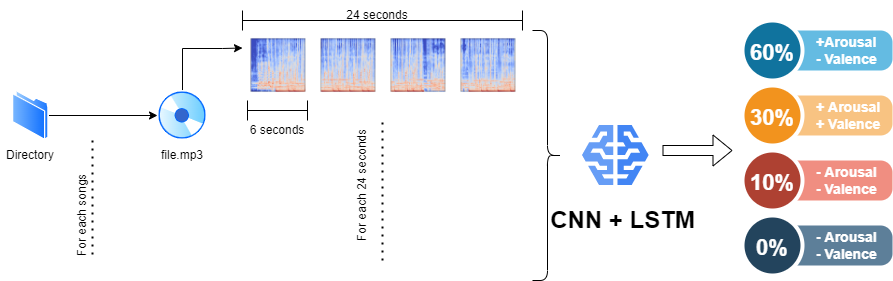
\includegraphics[scale = 0.45]{img/evaluation.png}
\caption{Summary of the final model applied to entire songs.}
\label{fig-user-evaluation}
\end{figure}





\begin{table}
\caption{Evaluation based on three subjects.}
\label{tab3}
\centering
\begin{tabular}{|c|c|c|c|c|}
\hline
 \textbf{Subject} & \textbf{User-Tuning} &  \textbf{Correct classification} & \textbf{Accuracy \%}  & \textbf{Average Difference Error}\\
\hline
&No Emotions Suggested &  24  & 0.48 & 40.03\\
 \textbf{1}&10 Emotions Suggested &  36   & 0.72 & 34.92 \\
&20 Emotions Suggested &  41   & 0.82 & 25.29\\
\hline
&No Emotions Suggested &  23  & 0.46 & 47.73\\
 \textbf{2}&10 Emotions Suggested &  31  & 0.62 & 37.88\\
&20 Emotions Suggested &  38  & 0.76 & 31.80\\
\hline
&No Emotions Suggested &  20  & 0.40 & 45.83\\
 \textbf{3}&10 Emotions Suggested &  27  & 0.54 & 32.20\\
&20 Emotions Suggested &  35  & 0.70 & 34.43\\

\hline
\end{tabular}
\end{table}

\begin{table}
\caption{Average values for suggested emotions.}
\label{tab4}
\centering
\begin{tabular}{|c|c|c|c|}
\hline
\textbf{User-Tuning} &  \textbf{Correct classification} & \textbf{Accuracy \%}  & \textbf{Average Difference Error}\\
\hline
\textbf{No Emotions Suggested} &  22.34  & 0.45 & 44.62\\
\hline
\textbf{10 Emotions Suggested} &  31.33  & 0.63 & 35\\
\hline
\textbf{20 Emotions Suggested} &  38  & 0.76 & 30.51\\
\hline


\hline
\end{tabular}
\end{table}

\newpage


\section{Conclusions and Future Work}

In this paper we have focused on the possibility of applying a general MER system to individual users, obtaining a more functional personalized experience. The results obtained show the possibility to apply deep learning models to recognize emotions and adapt them through user-tuning. The proposed approach consists in using a state of the art CNN to extract the features from Mel spectrograms and a LSTM network as a classifier. The model could easily be integrated into a music recommender system, in order to create personalized mood-based playlists. The playlist would then be based on the user's true emotions and no longer on general labels made by third parties, improving the user experience. The results obtained are promising, however it is necessary to extend the study by considering more songs and applying the model to real users playlist. A further study could be done in the field of wearable computing, using bracelets for real-time recognition of the user's emotions. Through this system, the need to explicitly ask the user for the emotion felt in listening could be removed and recognized directly from the device, providing better data for user-tuning.


\bibliographystyle{splncs04}
\bibliography{bibliography}

\end{document}
